Um dynamisch später hinzugefügte Algorithmen auch in der Ein- und Ausgabe zu unterstützen, werden die Komponenten "`PluginLoader"' und "`Plugin"' verwendet. Der PluginLoader handhabt die Plugins und erstellt diese falls notwendig. Um dies zu tun, hat der PluginLoader Zugriff auf die Algorithmen. Somit kann der PluginLoader ein Plugin für die Eingabe von Parametern erzeugen, indem er sich von dem entsprechenden Algorithmus die Anzahl der benötigten Parameter ausgeben lässt. Analog kann der PluginLoader ein Plugin zur Ausgabe erzeugen, indem er sich zurückgeben lässt wie die Ausgabedaten aussehen und diese Anhand des gewünschten Ausgabeformats entweder als plain-text, html-text, JSON, PNG-Grafik oder SVG+XML-Grafik aufbereitet.\\

\begin{figure}[h]
\centering
	\vspace{-5pt}
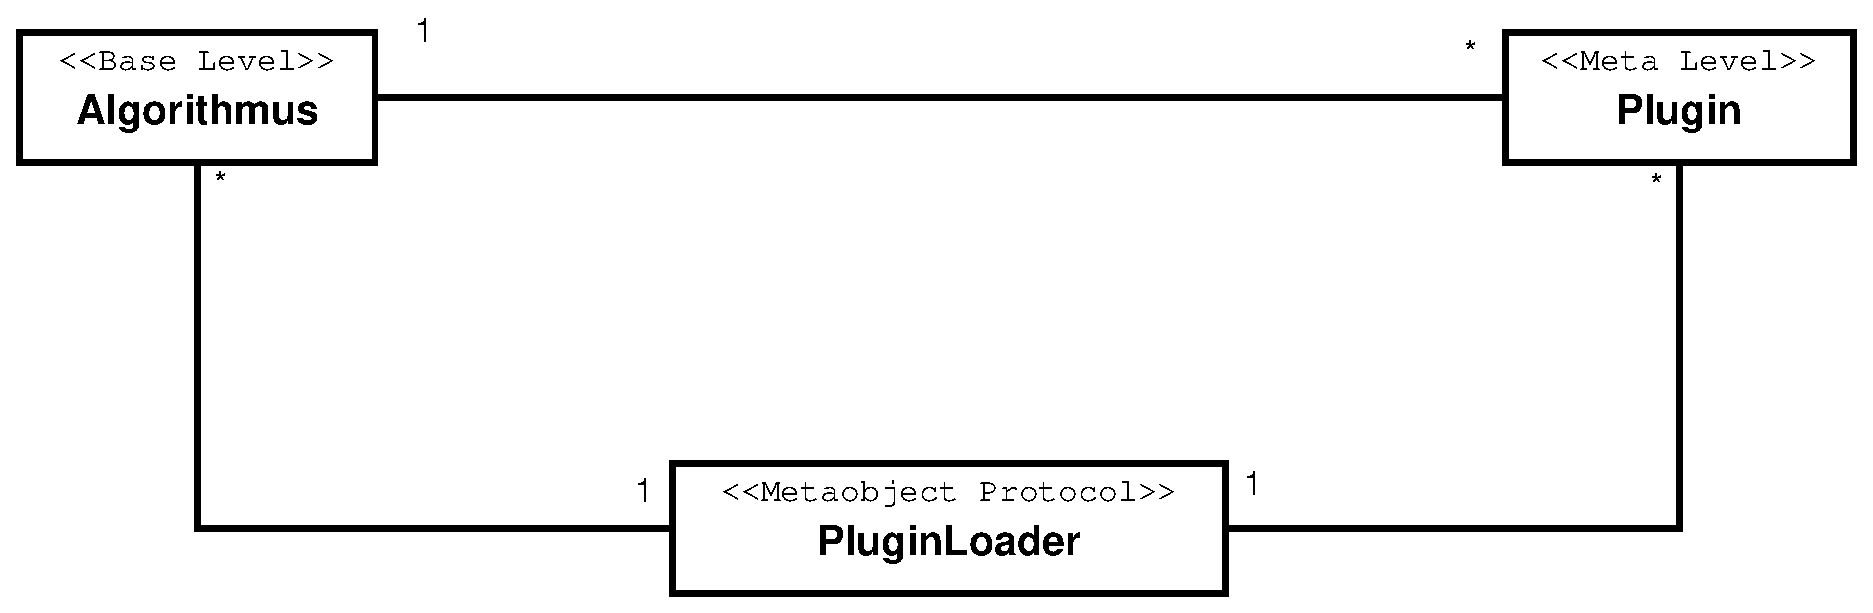
\includegraphics[width=0.7\linewidth]{Grafik/Diagramm/Reflection}
\caption[Reflection-Klasse]{Reflectoin-Pattern mit PluginLoader}
\label{fig:Reflection}
\end{figure}
\subsubsection{Was spricht für Reflection?}
Da das System ständig mit Algorithmen erweiterbar sein soll, wäre es hinderlich, wenn jede Eingabe- und Ausgabemaske für die Algorithmen extra geschrieben werden müssten. Deshalb ist es sinnvoll mithilfe des PluginLoaders diese Masken dynamisch mithilfe der Eingenschaften der Algorithmen zu erzeugen und als Plugins zu speichern. Soll nun das Design der Webseite angepasst werden, eine neue Ausgabe möglich sein oder eine andere Sprache unterstützt werden, so reicht eine Anpassung des PluginLoaders, um passende neue Plugins zu erstellen. Die Permance-Verluste sind an dieser Stelle akzeptabel, da keine Umfangreichen Operationen durchgeführt werden müssen, um den Prozess auszuführen. Auch eine ungewollte Manipulation ist auszuschließen, da der Zugriff auf die Komponenten des System durch den Nutzer sehr stark limitiert ist.

